%   Filename    : chapter_4.tex 
\chapter{System Architecture and Model Evaluation}
\section{System Architecture}
Using the tools mentioned in Section~\ref{sec:devtools}, our system can be visualized as shown in Figure \ref{fig:architecture}: 
\begin{figure}[h] % 'h' places the figure approximately here in the text
	\centering
	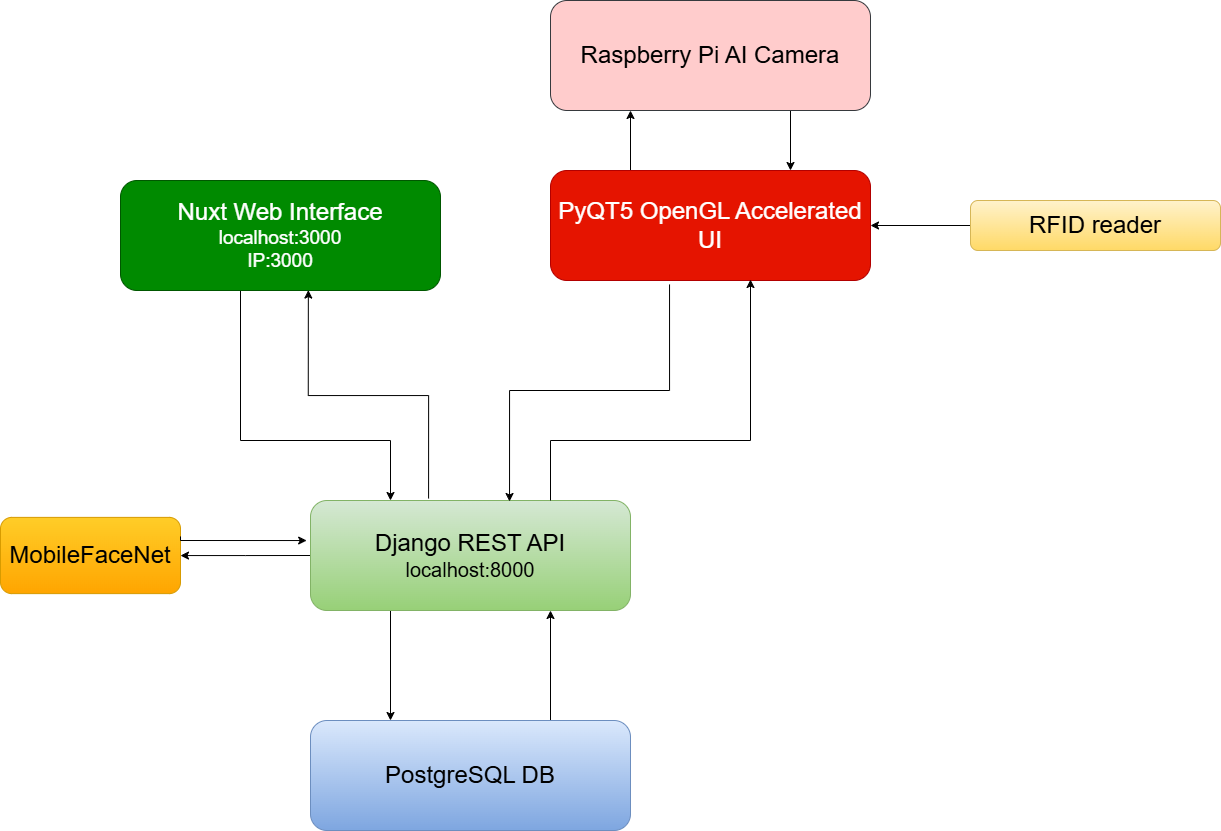
\includegraphics[width=0.55\textwidth]{figures/chapter4/architecture_new.png} % Adjust width as needed
	\caption{System Architecture}
	\label{fig:architecture}
\end{figure}

All software components and services are hosted on a Raspberry Pi 5.

We used Django as the backend server, which interfaces with the PostgreSQL database to perform queries in Python, because most pretrained facial recognition models are implemented in Python. We also used Django Ninja to allow the frontend to access backend data efficiently.

The frontend web interface is built using NuxtJS, which provides a comprehensive set of tools for routing, data fetching, and security. This interface is primarily used by faculty members to view and manage attendance records.

PyQt5 is used for interfacing with the Raspberry Pi AI Camera and the RFID scanner. It captures facial images and scans RFID tags. This component runs in a background thread to avoid interfering with the main web interface thread. PyQt5 initiates RFID scanning only when exactly one face is detected.

Once a face is successfully detected and an RFID tag is scanned, the captured facial image is encoded as a Base64 string and sent to the Django backend along with the RFID data. The backend uses MobileFaceNet to verify the identity by comparing the facial features and RFID information against existing records in the PostgreSQL database. If a match is found, the system logs the attendance.

The system has no online dependencies except for the Heroicons library, which is MIT-licensed and free to use.
\section{Use Case Discussion}

The use case diagram presented in Figure~\ref{fig:use_case} illustrates the primary interactions between system actors—\textbf{Teacher}, \textbf{Student}, and \textbf{Administrator}—and the core functionalities of the \textbf{UPTap Attendance System}. This diagram serves as a foundational blueprint for understanding the functional scope of the system and the responsibilities assigned to each user role.

\begin{figure}[h] % 'h' places the figure approximately here in the text
	\centering
	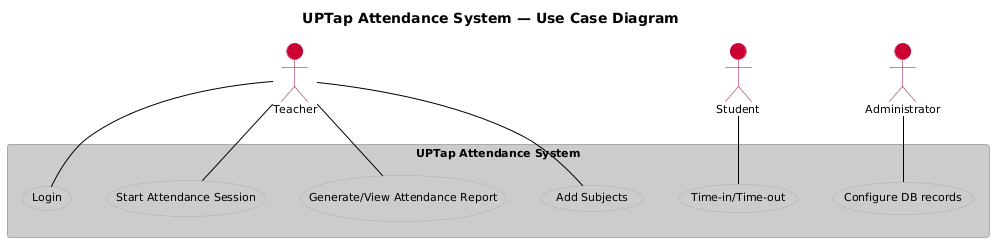
\includegraphics[width=1\textwidth]{figures/chapter4/use_case_diagram.png} % Adjust width as needed
	\caption{Use cases of the system. Generated using PlantUML.}
	\label{fig:use_case}
\end{figure}
\clearpage

\subsection*{Actors and Their Roles}

\begin{itemize}
	\item \textbf{Teacher}: The teacher has the most extensive set of interactions within the system. After logging in, the teacher initiates an attendance session, enabling students to time in or out during the allotted class period. Teachers can also add the subjects they handle, within the constraints of available time slots. Furthermore, they are able to generate or view attendance reports, allowing them to monitor class participation and maintain academic records.
	
	\item \textbf{Student}: The student's role is streamlined to support an efficient and automated attendance mechanism. Their primary interaction with the system is through the \textit{Time-in/Time-out} function, triggered via RFID. This design minimizes manual input, reduces errors, and promotes non-disruptive logging of attendance.
	
	\item \textbf{Administrator}: The administrator is responsible for configuring the system’s database records. This includes managing user accounts, setting up academic structures, and maintaining scheduling data. Although administrators do not participate directly in the attendance workflow, they provide critical backend support to ensure data consistency and system integrity.
\end{itemize}

\subsection*{Use Case Interactions}

Each use case has been designed to reflect real-world workflows:

\begin{itemize}
	\item \textbf{Login}: Ensures secure and role-based access to the system for teachers.
	\item \textbf{Start Attendance Session}: Enables teachers to activate the session during which students may time in. This supports token-based validation to prevent unauthorized entries.
	\item \textbf{Add Subjects}: Allows teachers to register the subjects they handle, with respect to available scheduling windows.
	\item \textbf{Generate/View Attendance Report}: Provides teachers access to attendance data for monitoring and reporting purposes.
	\item \textbf{Time-in/Time-out}: Represents the students’ main interaction, capturing presence data in a non-intrusive, automated manner.
	\item \textbf{Configure DB Records}: Reserved for administrators to manage database records, ensuring the structural integrity of the system.
\end{itemize}

\section{Process Diagrams }
\subsection{Overview of Process Flow}
The UPTap process flow diagram in Figure \ref{fig:flow} models the core interactions between the primary stakeholders in the attendance management system: teachers, students, and administrators. Each stakeholder's flow is represented as an independent, concurrent process, reflecting the real-world scenario where user roles interact with the system asynchronously.

\begin{figure}[h] % 'h' places the figure approximately here in the text
	\centering
	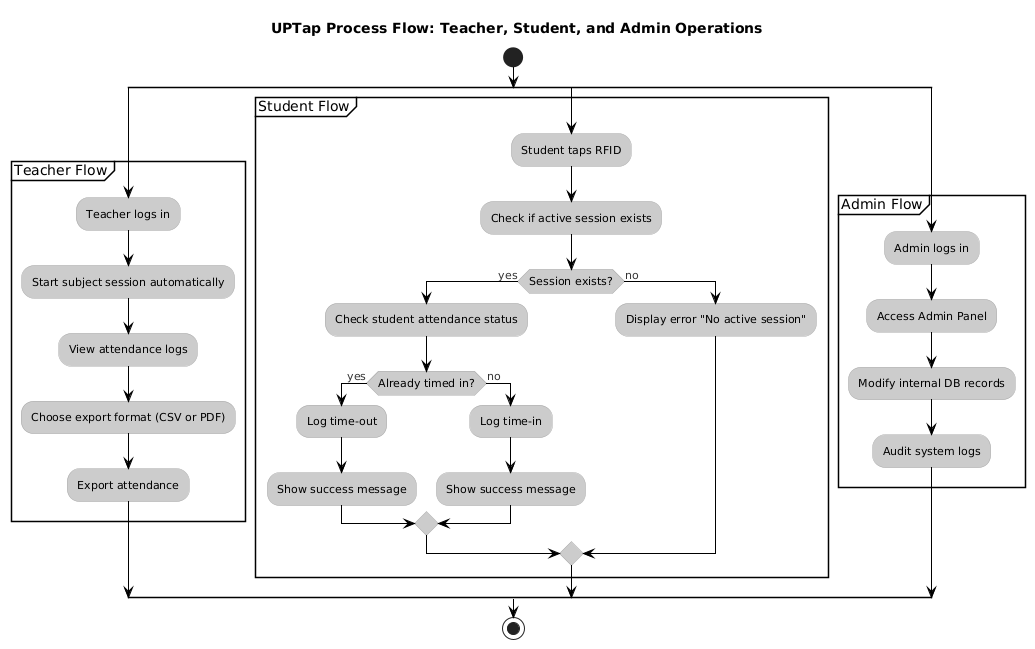
\includegraphics[width=1\textwidth]{figures/chapter4/flow.png} % Adjust width as needed
	\caption{The system process flow diagram. Generated using PlantUML.}
	\label{fig:flow}
\end{figure}

The Teacher Flow begins with authentication, followed by the initiation of subject-specific attendance sessions. Once sessions are active, teachers gain access to attendance logs and are provided with options to export records in either CSV or PDF format. This supports record-keeping, analytics, and institutional reporting. The design prioritizes simplicity for educators, automating session handling and emphasizing ease of use in exporting data.

The Student Flow is optimized for minimal interaction. Upon tapping an RFID card, the system first checks for an active session. If found, it evaluates the student's current attendance status. Based on whether the student has already timed in, the system either logs a time-out or a new time-in event. A success message confirms the action. If no session is active, an error message informs the student.

The Admin Flow provides backend support and oversight. Administrators can log into the system to debug operational issues, modify attendance records directly in the database, and audit system logs. This functionality is critical for maintaining data integrity and handling edge cases, such as hardware malfunctions or incorrectly recorded attendance events. The admin role operates independently of regular user flows and is not intended for daily operation but rather for exception handling and system maintenance.

\subsection{Student Registration Process}
Students must register their facial ID to enable attendance verification. This registration process only captures one facial image, which will be used to identify the student during attendance tracking. It also takes all relevant info about the student, reflecting the fields given by the generated class list of CRS. It will be handled by Nuxt at endpoint: \url{http://raspberry_ip:3000/public/register}. Figures \ref{fig:student_form_pc} to \ref{fig:student_form_mobile_preview} detail the process.
\begin{figure}[h] % 'h' places the figure approximately here in the text
	\centering
	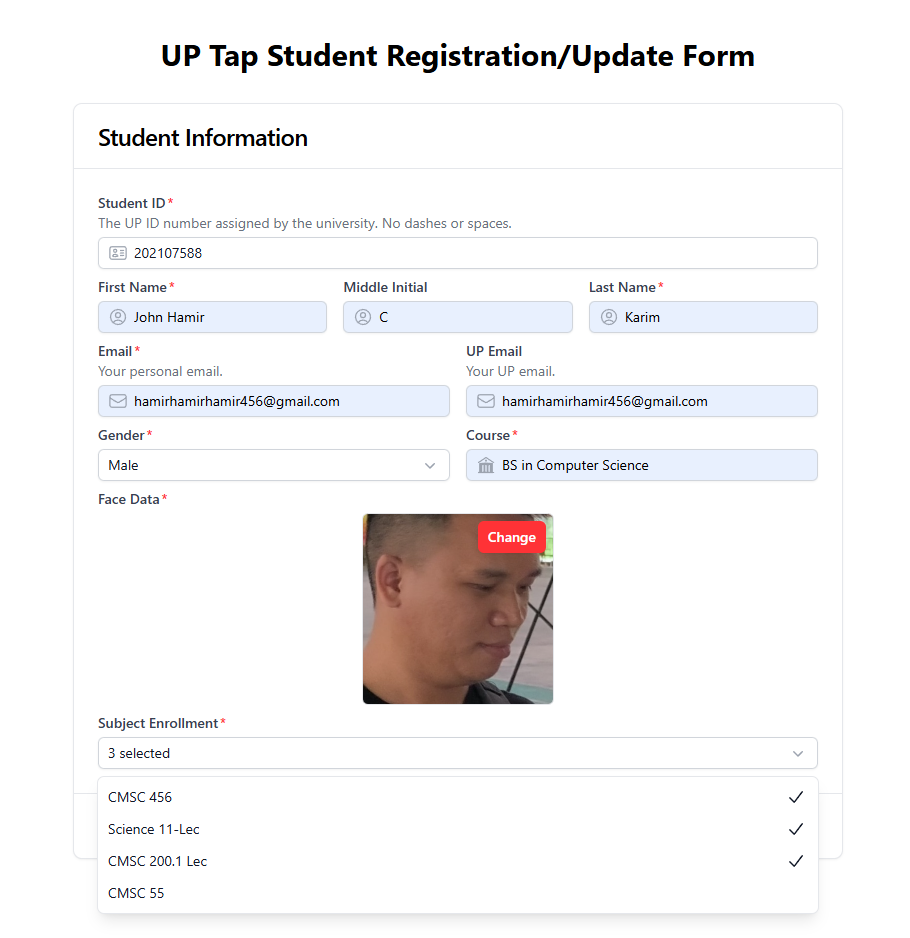
\includegraphics[width=0.75\textwidth]{figures/chapter4/student_form_pc.png} % Adjust width as needed
	\caption{Form in desktop client. Face data defaults to file picker. It will still check for faces in the image. Course input lists all courses offered in UP Visayas.}
	\label{fig:student_form_pc}
\end{figure}
\clearpage

\begin{figure}[h] % 'h' places the figure approximately here in the text
	\centering
	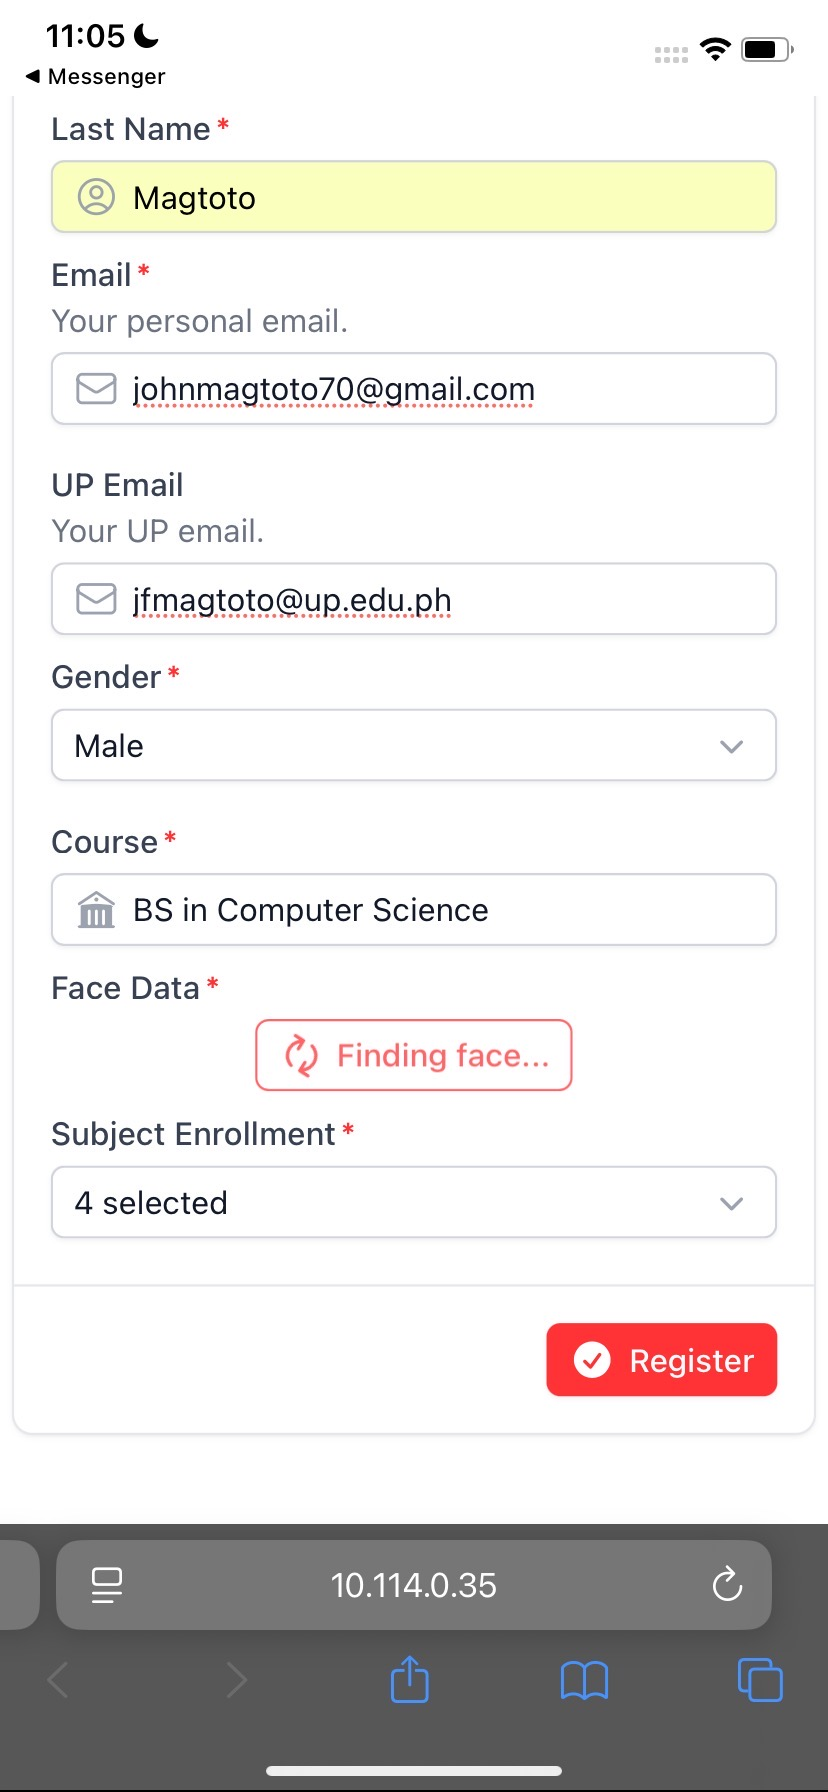
\includegraphics[width=0.5\textwidth]{figures/chapter4/student_form_mobile.jpg} % Adjust width as needed
	\caption{Form in mobile devices. Face data will use the native camera instead. It will then detect faces from the image provided.}
	\label{fig:student_form_mobile}
\end{figure}
\clearpage
\begin{figure}[h] % 'h' places the figure approximately here in the text
	\centering
	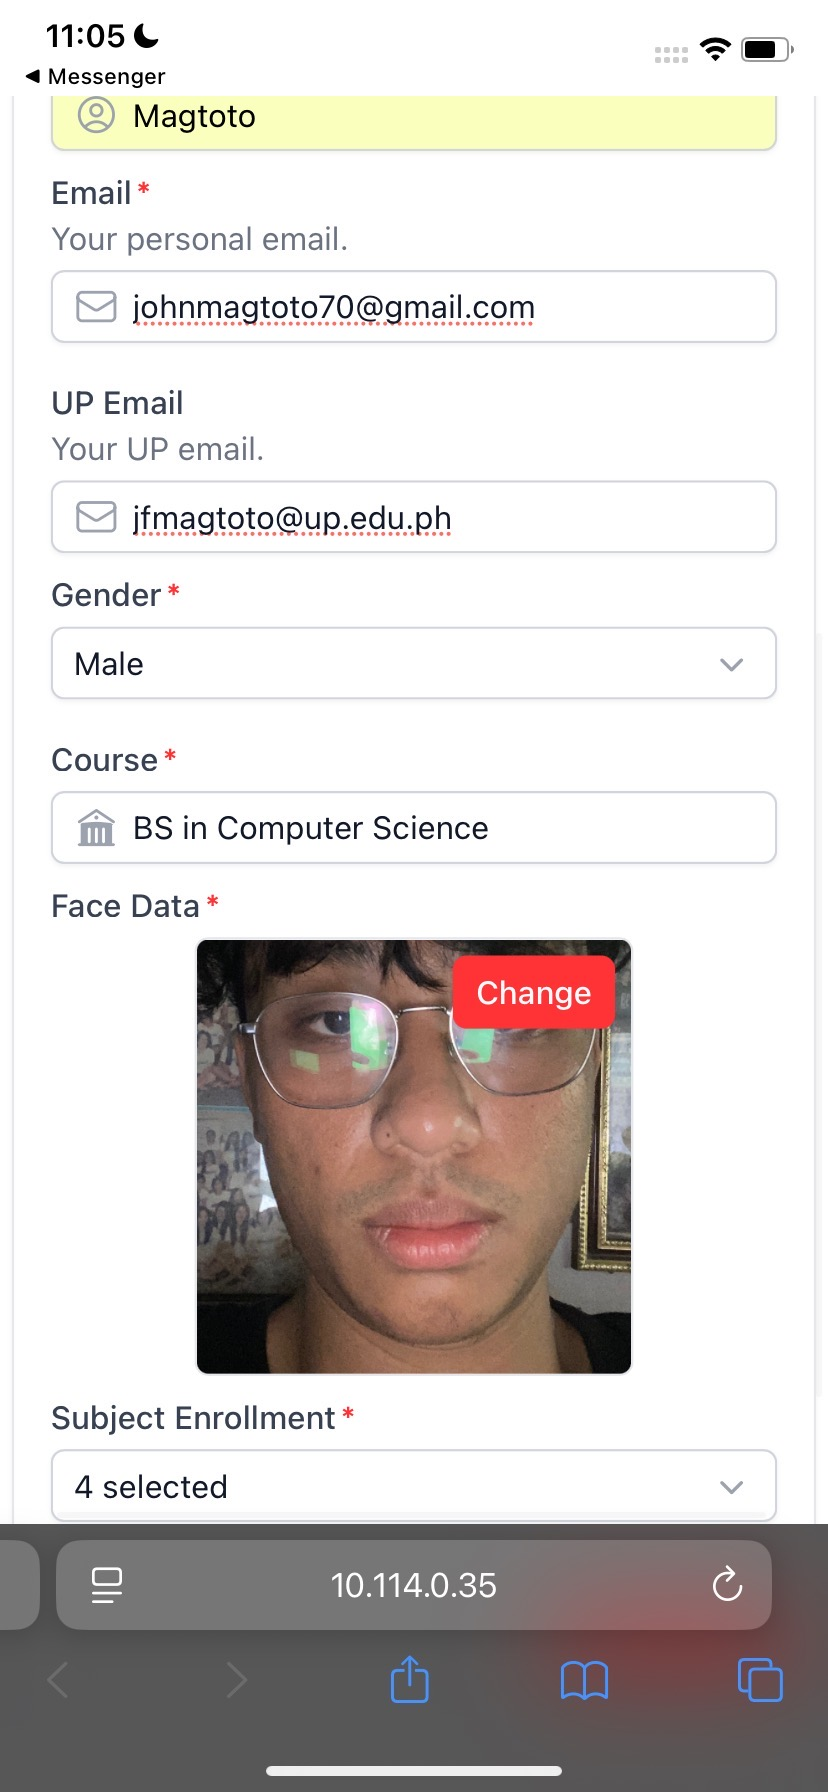
\includegraphics[width=0.5\textwidth]{figures/chapter4/student_form_mobile_preview.jpg} % Adjust width as needed
	\caption{Face data preview when face is detected. Otherwise show an alert window for image retake.}
	\label{fig:student_form_mobile_preview}
\end{figure}
\clearpage
\subsection{Time In Process}
Time in process includes a check if the student already has time in records. First step in this is the student tapping the ID to the RFID sensor and trigger the photo capture to check the face. The system also checks if the time-in request happened within the subject time slot and session which the student is enrolled to. If we satisfy these conditions, we log the attendance information to the database, and the backend server sends a server side event to update the frontend records in real time.
\begin{figure}[h] % 'h' places the figure approximately here in the text
	\centering
	\includegraphics[width=1.0\textwidth]{figures/chapter4/Timein2.png} % Adjust width as needed
	\caption{Time In process. Checks if there's already a time in record.}
	\label{fig:timein}
\end{figure}

\clearpage
\subsection{Time Out Process}
The time out process is the same as time-in process, we just update the time-out column of the attendance information table.
\begin{figure}[h] % 'h' places the figure approximately here in the text
	\centering
	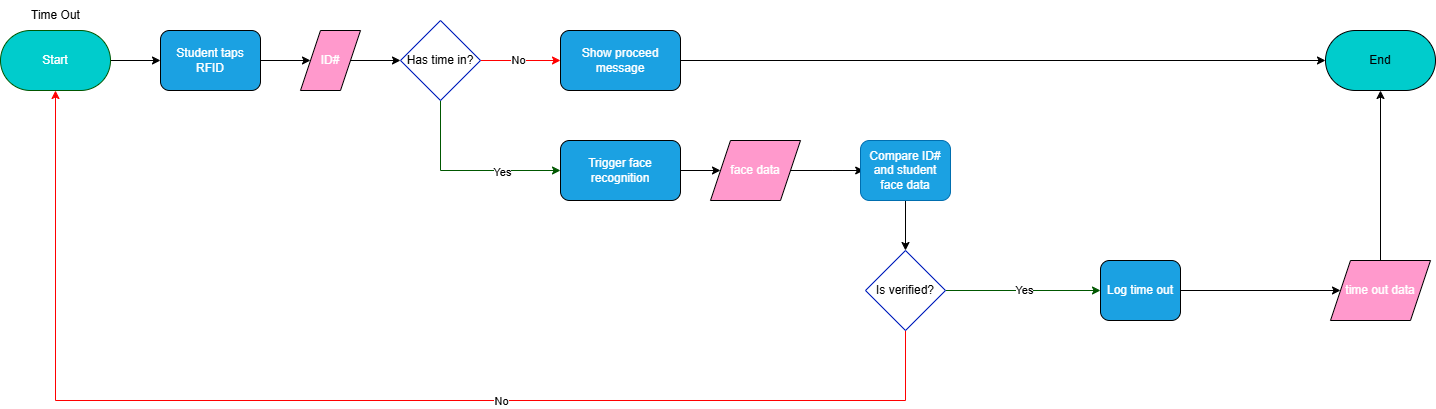
\includegraphics[width=1.0\textwidth]{figures/chapter4/timeout1.png} % Adjust width as needed
	\caption{Time Out}
	\label{fig:timeout}
\end{figure}

\subsection{Attendance Record Export Process}
The faculty members are allowed to export their attendance records into a CSV/PDF file in order to have better access and record keeping. In addition to that, this feature can be useful for further analysis, for data backup purposes, or if they want to integrate it into another academic system. Figure \ref{fig:att_ui} show the UI for the attendance records, with a button on the left for export options. Figure \ref{fig:att_report} shows the generated report PDF.
\begin{figure}[h] % 'h' places the figure approximately here in the text
	\centering
	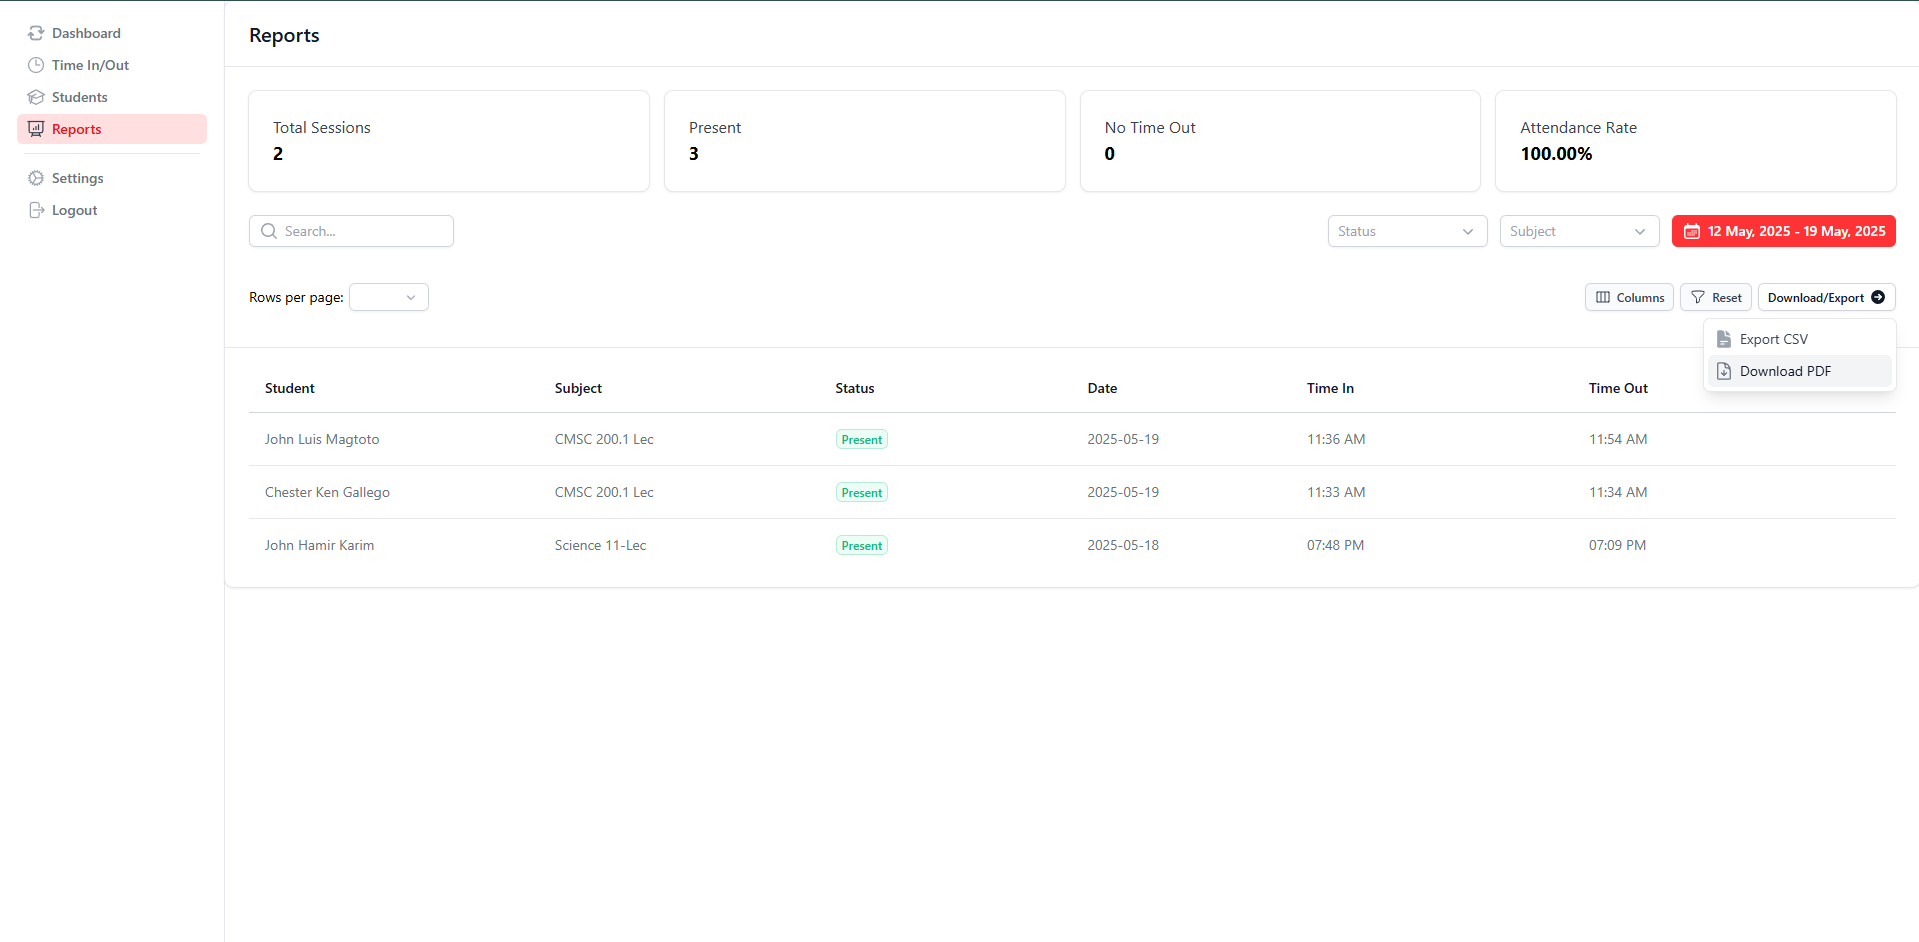
\includegraphics[width=1.0\textwidth]{figures/chapter4/att_ui.png} % Adjust width as needed
	\caption{Reports page}
	\label{fig:att_ui}
\end{figure}
\begin{figure}[h] % 'h' places the figure approximately here in the text
	\centering
	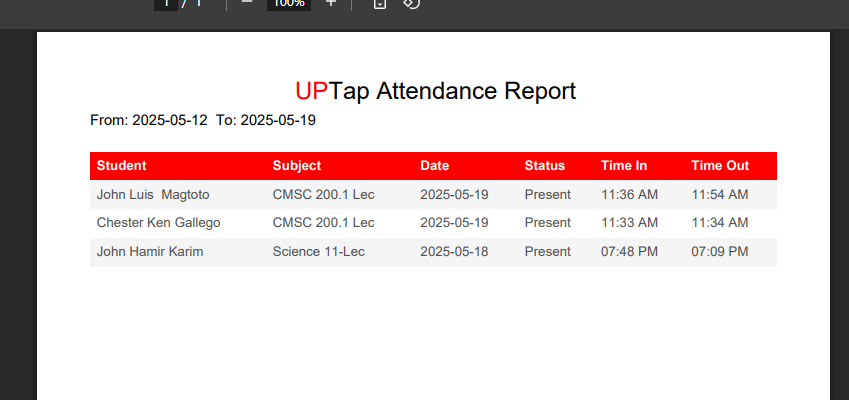
\includegraphics[width=1.0\textwidth]{figures/chapter4/att_report.png} % Adjust width as needed
	\caption{Report PDF}
	\label{fig:att_report}
\end{figure}
\clearpage
\section{Django Backend}
\subsection{Models}
Django Model class maps to SQL tables. For example, a Student table will have the following columns which maps to Student Model class' attributes like in Figure \ref{fig:models}: 

\begin{figure}[h] % 'h' places the figure approximately here in the text
	\centering
	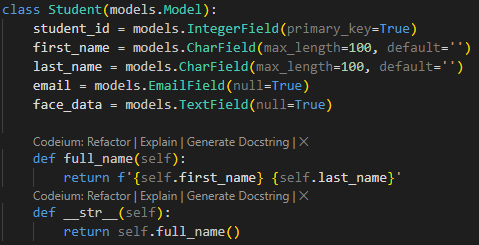
\includegraphics[width=0.8\textwidth]{figures/chapter4/models.png} % Adjust width as needed
	\caption{Student model}
	\label{fig:models}
\end{figure}

SQL equivalent would be:
\begin{verbatim}
	CREATE TABLE Student (
	student_id INTEGER PRIMARY KEY,
	first_name VARCHAR(100) NOT NULL DEFAULT '',
	last_name VARCHAR(100) NOT NULL DEFAULT '',
	email VARCHAR(254),
	face_data TEXT,
	CONSTRAINT unique_email UNIQUE (email)
	);
\end{verbatim}
\subsection{Database Table}
The database tables are automatically generated using django-extensions module. It reads all the Model classes in our Django project and generates the connections between tables.
\begin{figure}[h] % 'h' places the figure approximately here in the text
	\centering
	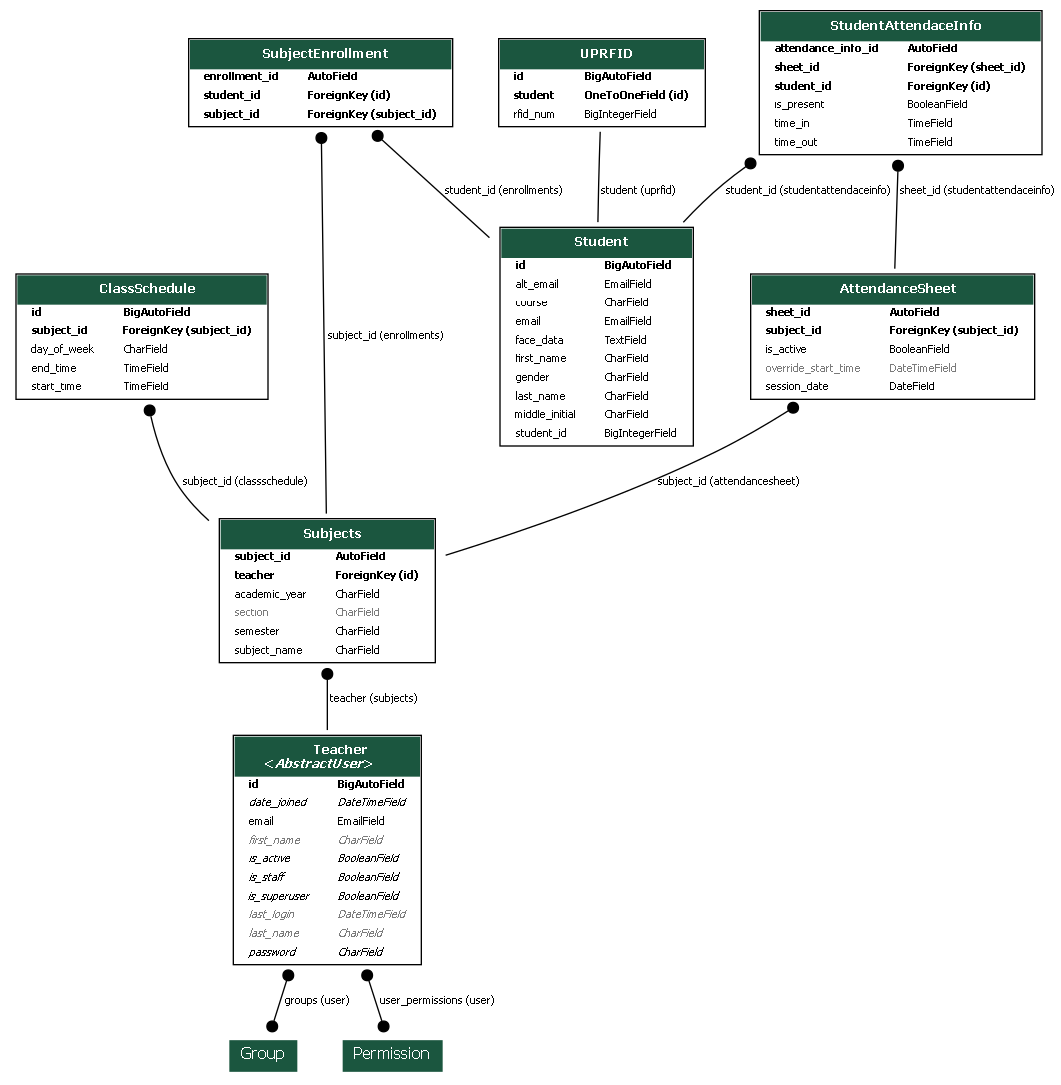
\includegraphics[width=1\textwidth]{figures/chapter4/auto_erd.png} % Adjust width as needed
	\caption{System Architecture}
	\label{fig:db_tables}
\end{figure}	

\subsection{REST API by Django Ninja}
Figure~\ref{fig:api} is the automatic OpenAPI compliant documentation provided by Django Ninja. It contains all endpoints we can use to query data from the database. All endpoints are protected using HTTP Bearer token authentication.
\begin{figure}[h] % 'h' places the figure approximately here in the text
	\centering
	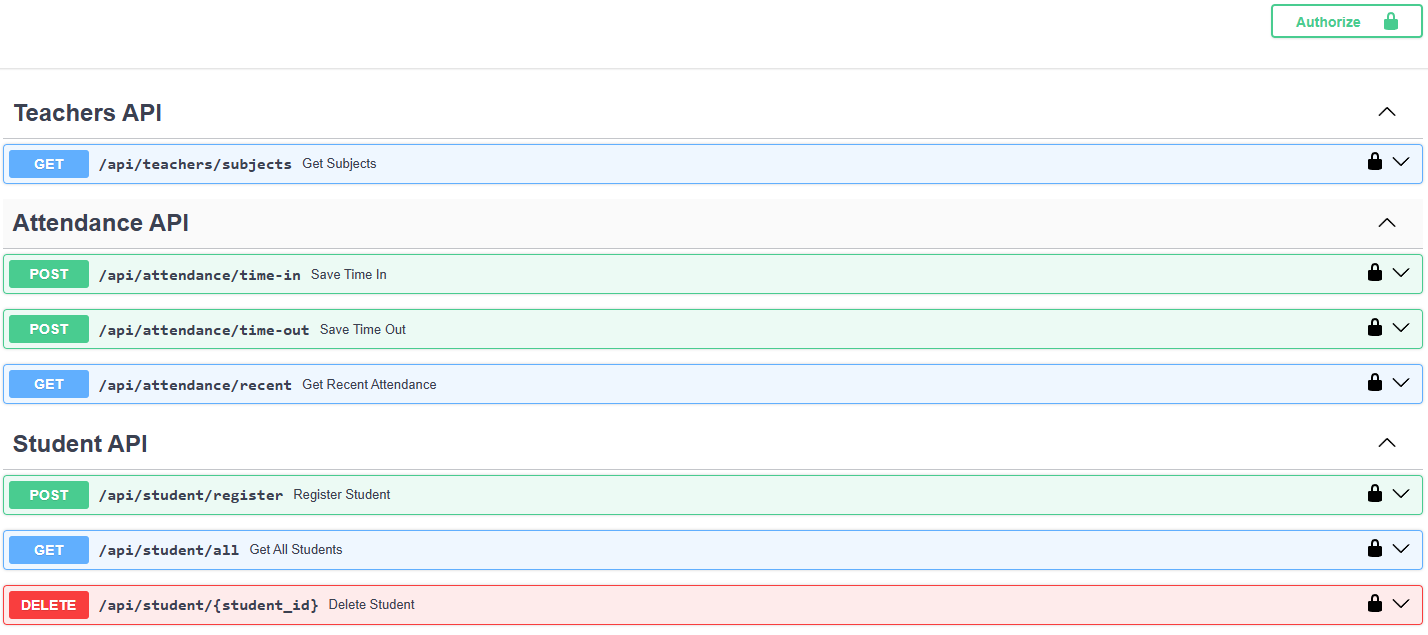
\includegraphics[width=1\textwidth]{figures/chapter4/api.png} % Adjust width as needed
	\caption{API Documentation}
	\label{fig:api}
\end{figure}

\subsection{Admin panel by Django}
Figure~\ref{fig:admin} is the Django administration page only accessible to a superuser account. This is where most of the backend maintanance work happens. It contains all the data inside the database allow full control over them. It also contains every authentication tokens used by each teacher account.
\begin{figure}[h] % 'h' places the figure approximately here in the text
	\centering
	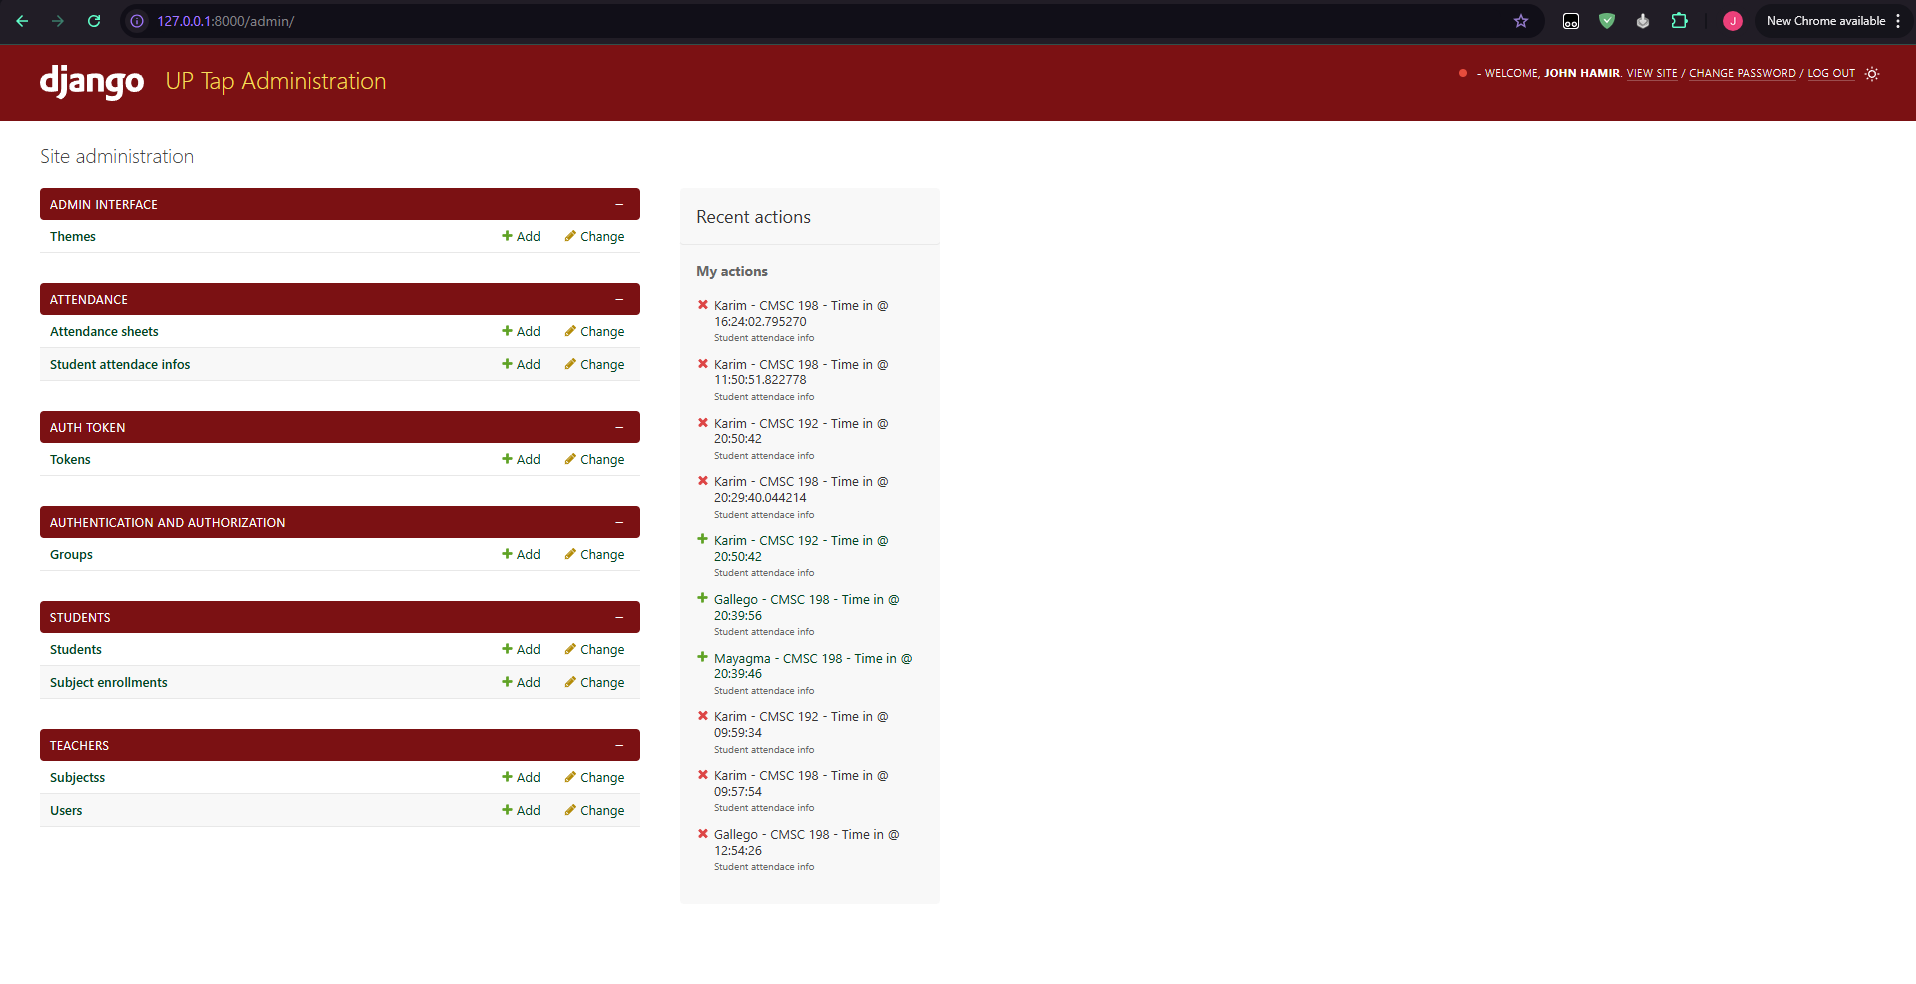
\includegraphics[width=1\textwidth]{figures/chapter4/admin.png} % Adjust width as needed
	\caption{Django Administration}
	\label{fig:admin}
\end{figure}

\section{Nuxt Frontend}
The Nuxt web interface functions as the main UI with out system. It handles faculty onboarding and CSV imports of their class list from the CRS. It also has student management system for the basic CRUD operations for students' information.
\subsection{Faculty Onboarding}
The faculty must register using their email and personal details to use the system. We can verify the authenticity of the email by sending them a link that activates the newly created account. After the registration process, they can now log in and use the system.
\begin{figure}[h] % 'h' places the figure approximately here in the text
	\centering
	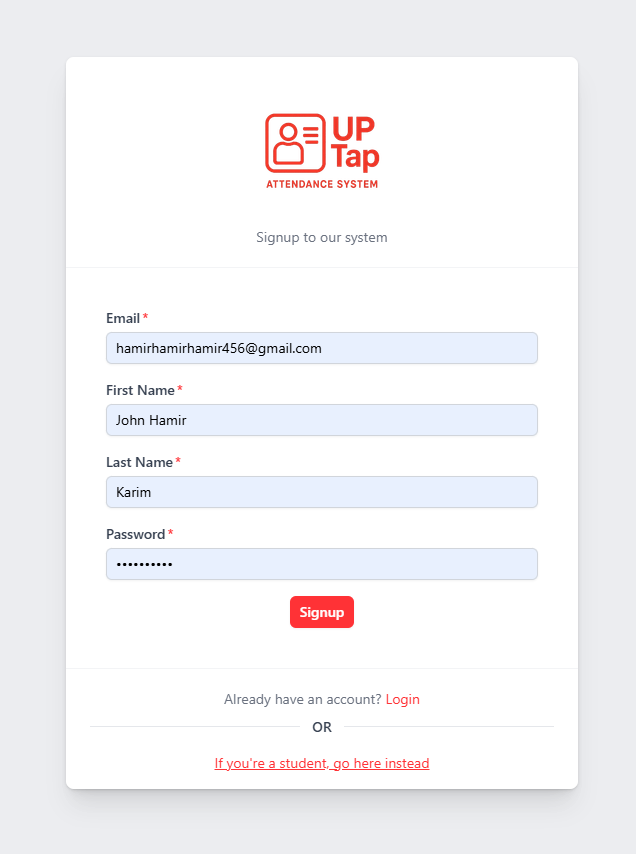
\includegraphics[width=0.8\textwidth]{figures/chapter4/faculty_signup.png} % Adjust width as needed
	\caption{Faculty Signup using email, first name, and last name}
	\label{fig:faculty_signup}
\end{figure}
\clearpage
\begin{figure}[h] % 'h' places the figure approximately here in the text
	\centering
	
\includegraphics[width=0.8\textwidth]{figures/chapter4/faculty_signup_info.png} % Adjust width as needed
	\caption{Notice after new signup}
	\label{fig:faculty_signup_info}
\end{figure}
\begin{figure}[h] % 'h' places the figure approximately here in the text
	\centering
	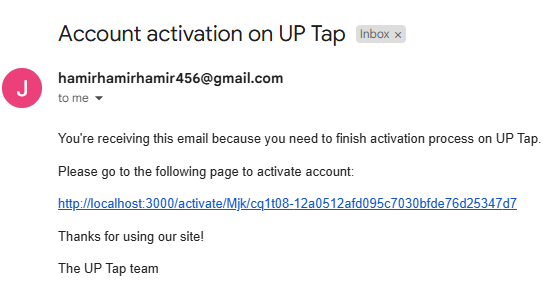
\includegraphics[width=0.8\textwidth]{figures/chapter4/faculty_signup_email.png} % Adjust width as needed
	\caption{Email containing the link for activation. Activation must be done on the same device.}
	\label{fig:faculty_signup_email}
\end{figure}
\begin{figure}[h] % 'h' places the figure approximately here in the text
	\centering
	
\includegraphics[width=0.8\textwidth]{figures/chapter4/faculty_activation.png} % Adjust width as needed
	\caption{Activating account on the link provided.}
	\label{fig:faculty_activation}
\end{figure}
\begin{figure}[h] % 'h' places the figure approximately here in the text
	\centering
	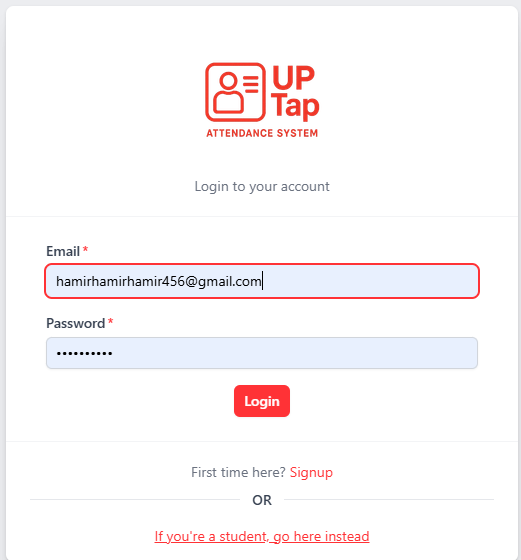
\includegraphics[width=0.8\textwidth]{figures/chapter4/faculty_login.png} % Adjust width as needed
	\caption{We can now login after opening the link.}
	\label{fig:faculty_login}
\end{figure}
\clearpage

\subsection{Subject CRUD Operations}
Subject creation is handled exclusively by the faculty members only with verified accounts. Each faculty is able to create subjects on their own, but it should not conflict with the time schedules of other faculty members. The system will warn for such conflicts. The modal for subject creation will provide a view of available time slots not taken by other subjects.
\begin{figure}[h] % 'h' places the figure approximately here in the text
	\centering
	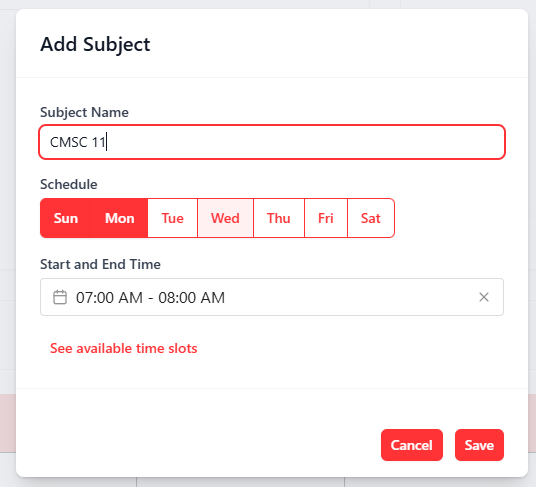
\includegraphics[width=0.8\textwidth]{figures/chapter4/subject_add.png} % Adjust width as needed
	\caption{Adding new subjects}
	\label{fig:subject_add}
\end{figure}
\begin{figure}[h] % 'h' places the figure approximately here in the text
	\centering
	
\includegraphics[width=0.8\textwidth]{figures/chapter4/subject_add_success.png} % Adjust width as needed
	\caption{Success}
	\label{fig:subject_add_success}
\end{figure}
\clearpage
\begin{figure}[h] % 'h' places the figure approximately here in the text
	\centering
	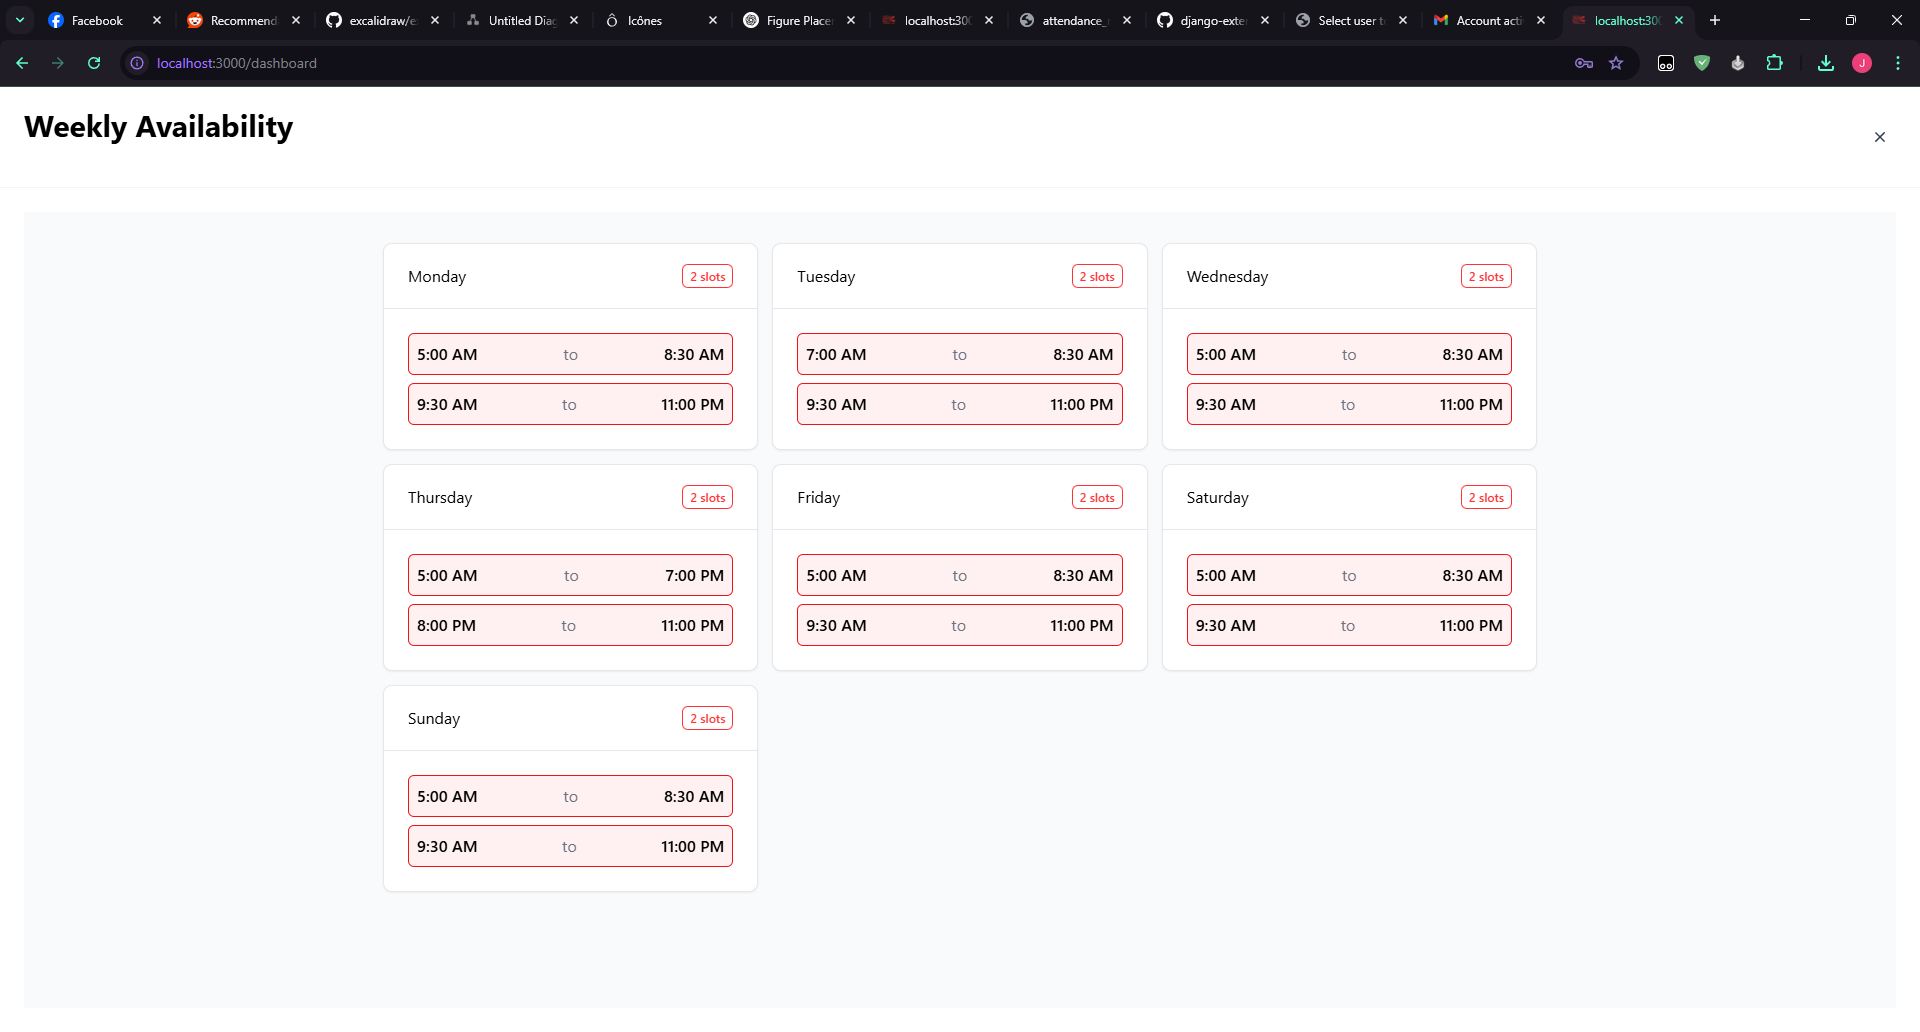
\includegraphics[width=0.8\textwidth]{figures/chapter4/subject_availability.png} % Adjust width as needed
	\caption{Available slots}
	\label{fig:subject_availability}
\end{figure}
\begin{figure}[h] % 'h' places the figure approximately here in the text
	\centering
	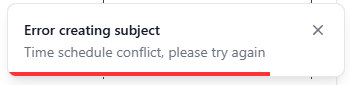
\includegraphics[width=0.8\textwidth]{figures/chapter4/subject_add_error.png} % Adjust width as needed
	\caption{Error due to time conflict}
	\label{fig:subject_add_error}
\end{figure}
\subsection{Faculty CSV Import Process}
After adding subjects, we can now import class list in CSV format. The faculty members can upload a CSV file containing the students' details. The system parses the CSV file and stores the extracted data in the database. The data uploaded is validated to avoid any duplicate or wrong entries. The backend populates/updates the Student table with the data and creates entries in the SubjectEnrollment table to tie each Student to a Subject. See Figure \ref{fig:faculty_import}
\begin{figure}[h] % 'h' places the figure approximately here in the text
	\centering
	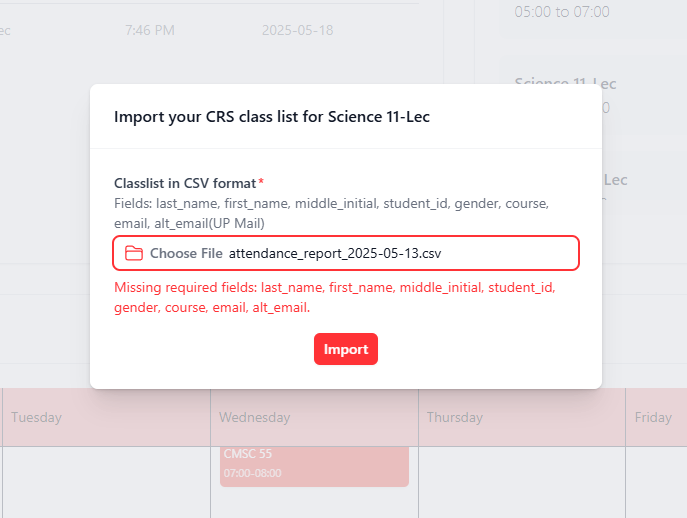
\includegraphics[width=0.8\textwidth]{figures/chapter4/faculty_import.png} % Adjust width as needed
	\caption{Faculty Import using CSV}
	\label{fig:faculty_import}
\end{figure}
\begin{figure}[h] % 'h' places the figure approximately here in the text
	\centering
	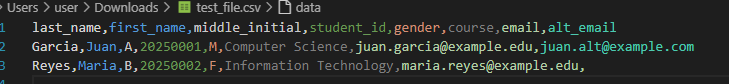
\includegraphics[width=0.8\textwidth]{figures/chapter4/faculty_import_csv.png} % Adjust width as needed
	\caption{CSV sample file}
	\label{fig:faculty_import_csv}
\end{figure}
\begin{figure}[h] % 'h' places the figure approximately here in the text
	\centering
	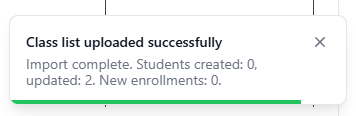
\includegraphics[width=0.8\textwidth]{figures/chapter4/faculty_import_success.png} % Adjust width as needed
	\caption{Import success}
	\label{fig:faculty_import_success}
\end{figure}
\clearpage
\subsection{Students CRUD operations}
By default, the \url{/students} tab will list all students under the logged in teacher.
\begin{figure}[h] % 'h' places the figure approximately here in the text
	\centering
	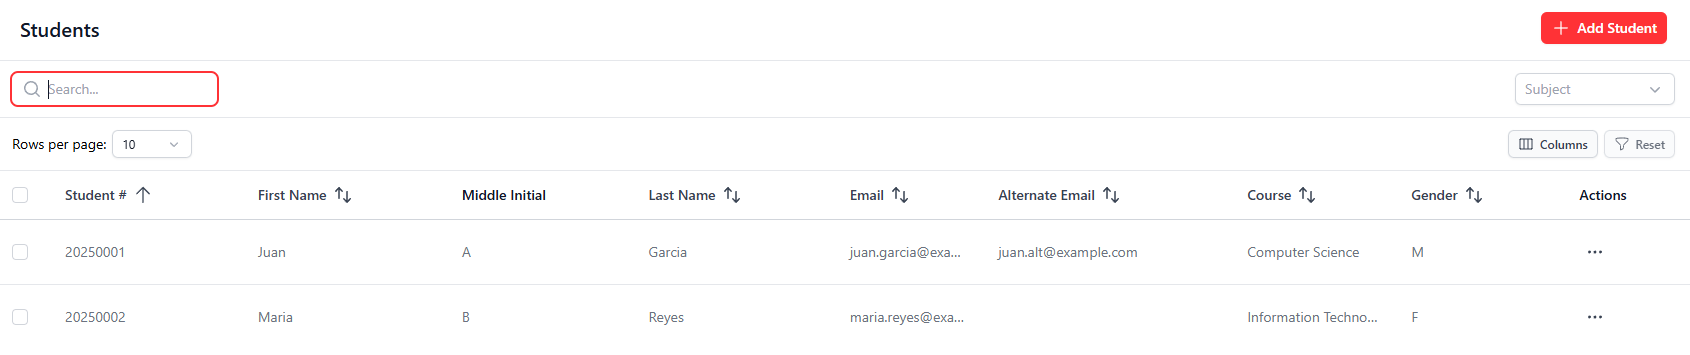
\includegraphics[width=1\textwidth]{figures/chapter4/student_list.png} % Adjust width as needed
	\caption{Students page}
	\label{fig:student_list}
\end{figure}
At this point, we still don't have information about the RFID of the student. We can add them by batch in this page. Connect the RFID scanner and scan the matching ID. The web app will wait for key events and automatically save the RFID of students scanned.
\begin{figure}[h] % 'h' places the figure approximately here in the text
	\centering
	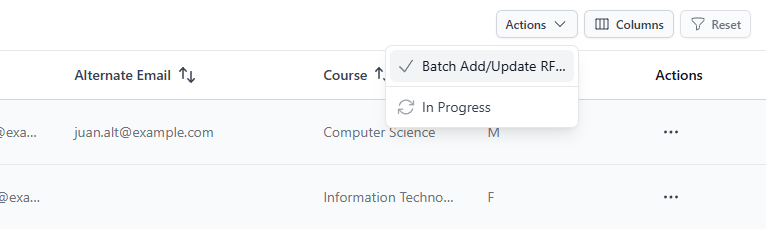
\includegraphics[width=1\textwidth]{figures/chapter4/batch_rfid.png} % Adjust width as needed
	\caption{Batch Actions}
	\label{fig:batch_rfid}
\end{figure}
\begin{figure}[h] % 'h' places the figure approximately here in the text
	\centering
	
\includegraphics[width=1\textwidth]{figures/chapter4/batch_rfid_scan.png} % Adjust width as needed
	\caption{Automatic scanner. The faculty do not need to press anything, as the scanner simulates an Enter press after scanning the RFID number.}
	\label{fig:batch_rfid_scan}
\end{figure}
\clearpage
\subsection{Web equivalent of the time-in and time-out process}
It also has a web equivalent of the PyQT5 time-in and time-out processing, albeit much slower. See Figures \ref{fig:faculty_import} and \ref{fig:frontend}.
\begin{figure}[h] % 'h' places the figure approximately here in the text
	\centering
	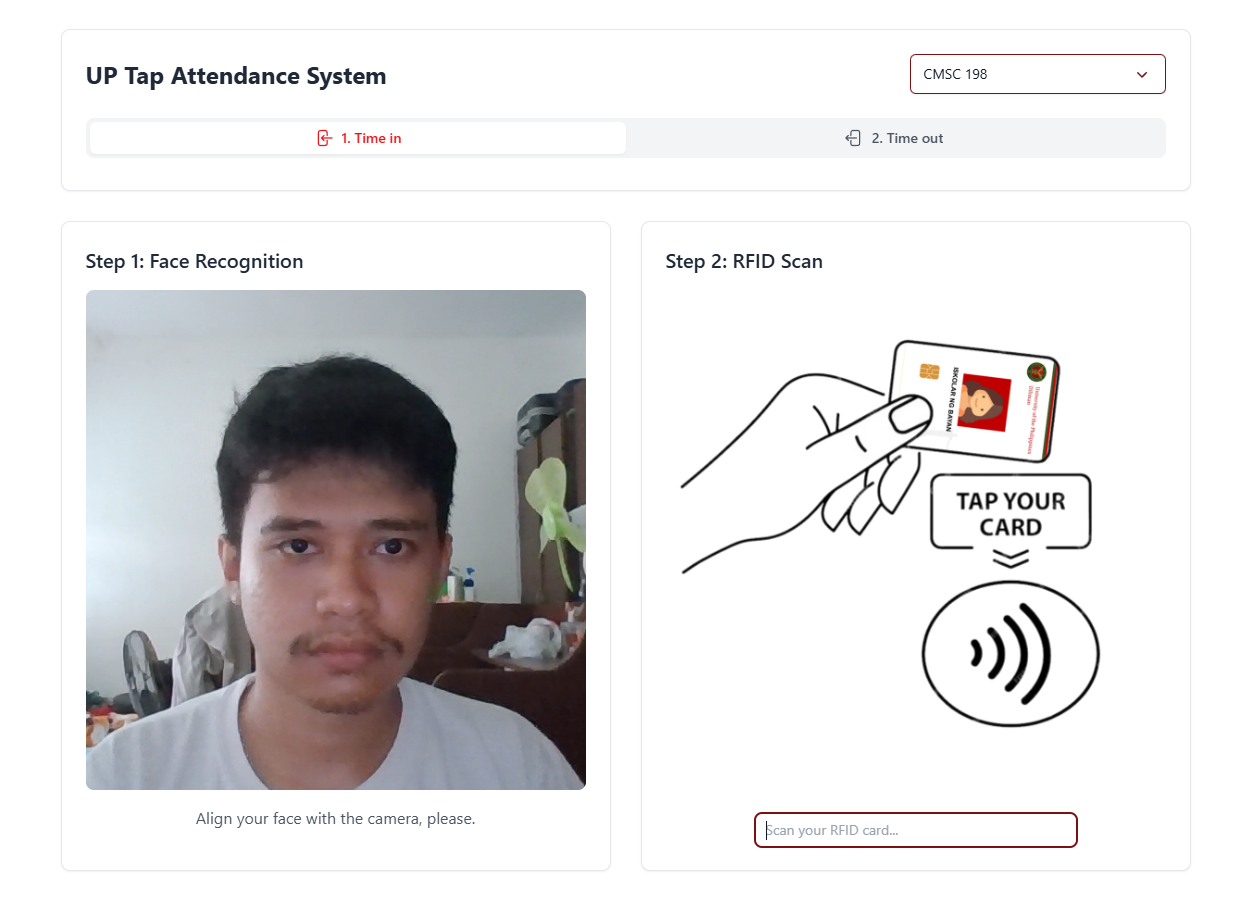
\includegraphics[width=1.0\textwidth]{figures/chapter4/frontend.png} % Adjust width as needed
	\caption{Time in and Time out Page}
	\label{fig:frontend}
\end{figure}

\begin{figure}[h] % 'h' places the figure approximately here in the text
	\centering
	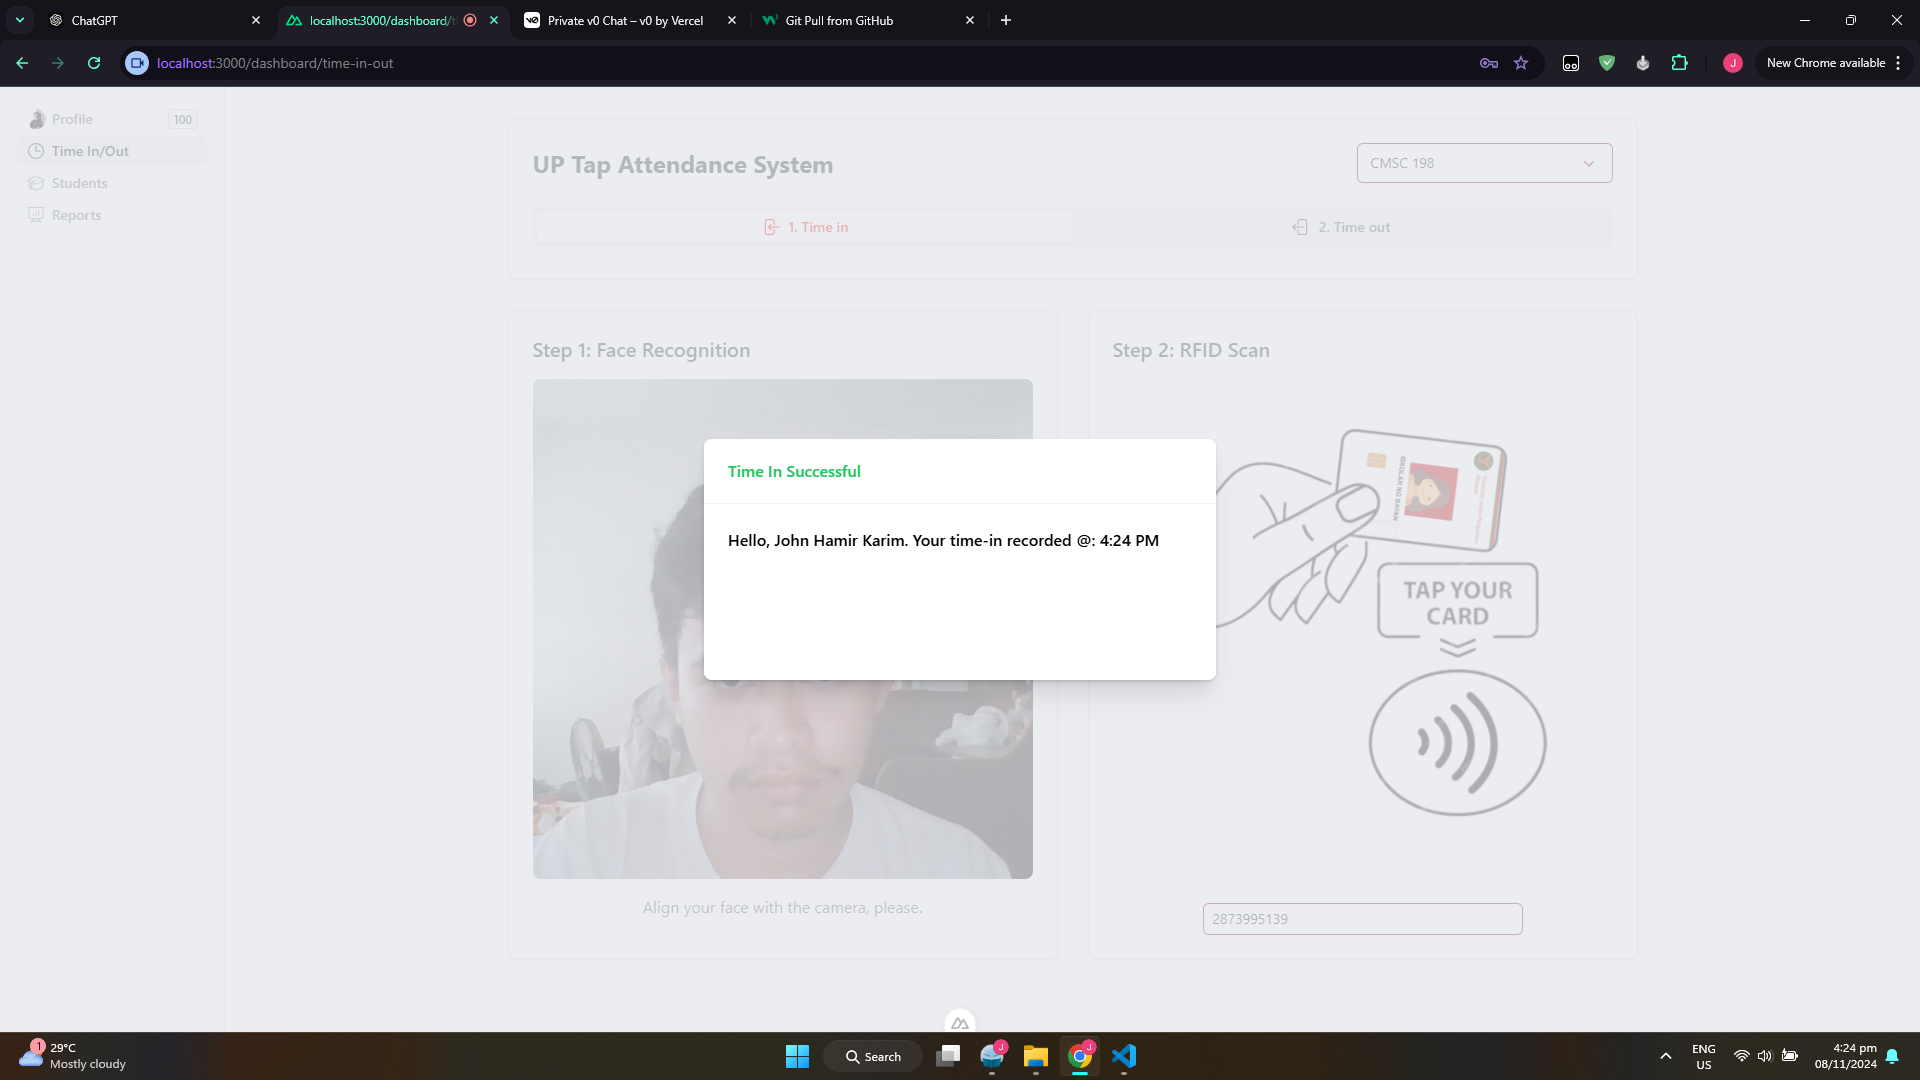
\includegraphics[width=1.0\textwidth]{figures/chapter4/success.png} % Adjust width as needed
	\caption{Successful Time In}
	\label{fig:success}
\end{figure}
\begin{figure}[h] % 'h' places the figure approximately here in the text
	\centering
	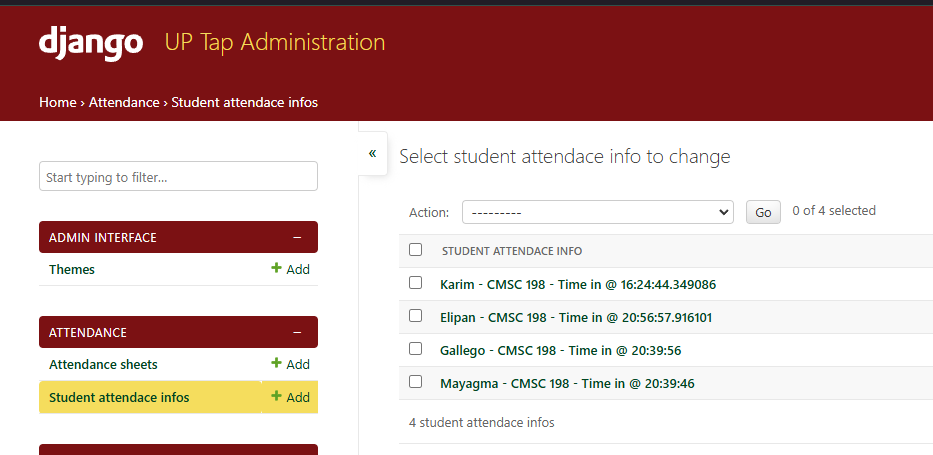
\includegraphics[width=0.75\textwidth]{figures/chapter4/backendrecord.png} % Adjust width as needed
	\caption{Django saving the attendance time instance in 24-hr format}
	\label{fig:record}
\end{figure}

\clearpage
\section{Raspeberry Pi AI Camera}
The AI camera is responsible for handling the face detection inference by running the compressed face detection model based on YoloV8n on the onboard Sony IMX500 chip. This takes off the workload of continuous streaming and inference from the Raspberry Pi 5 CPU/GPU and will allow it to scale better and allocate compute resources for other parts of the system such as the face verification and database operations.
\begin{figure}[h] % 'h' places the figure approximately here in the text
	\centering
	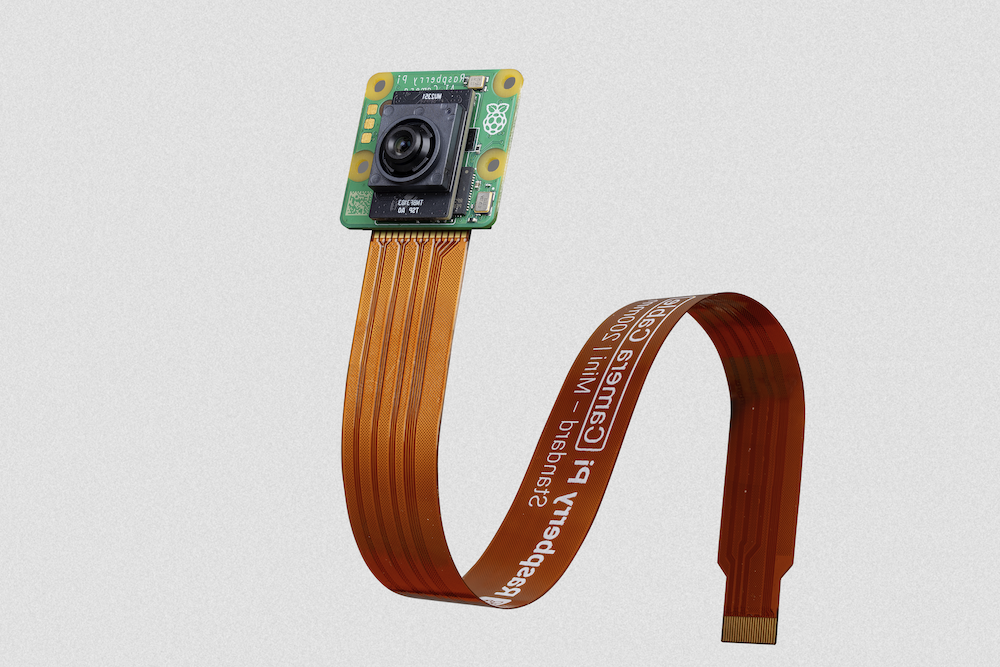
\includegraphics[width=0.75\textwidth]{figures/chapter4/ai_cam.png} % Adjust width as needed
	\caption{The AI camera has the Sony IMX500 in the same silicon.}
	\label{fig:ai_cam}
\end{figure}
\subsection{Comparison with traditional camera solutions for Raspberry devices}
The AI camera is not limited to object detection tasks like face detection. It is also capable of doing pose estimation, image classification, and object segmentation all on the same chip as the camera. This is a huge jump in technology compared to the earlier cameras for the Raspberry Pi ecosystem and eliminates the need for AI accelerators that are attached on top of the Raspberry Pi. Figure \ref{fig:ai_cam_comparison} compares the architecture or traditional cameras and the new AI camera. 
\begin{figure}[h] % 'h' places the figure approximately here in the text
	\centering
	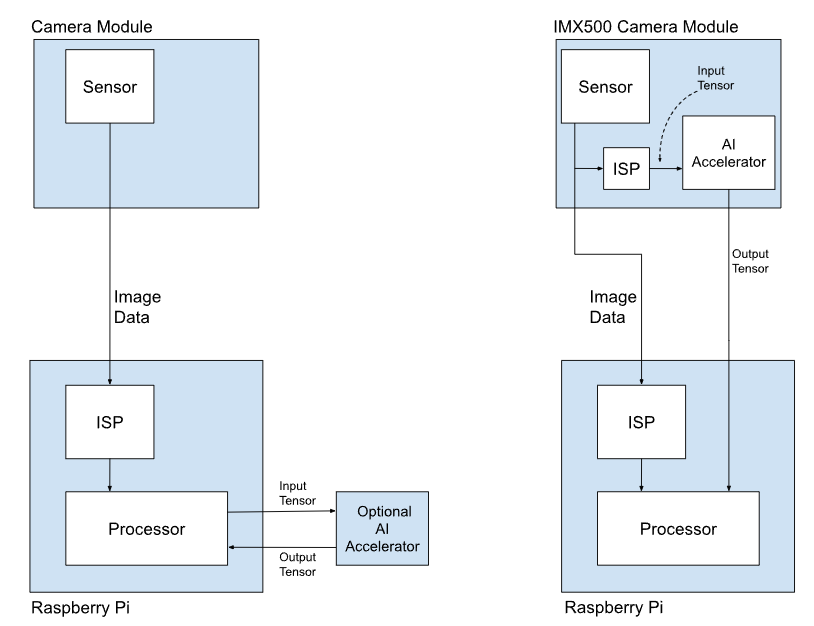
\includegraphics[width=0.75\textwidth]{figures/chapter4/ai_cam_comparison.png} % Adjust width as needed
	\caption{New AI camera vs Traditional Camera}
	\label{fig:ai_cam_comparison}
\end{figure}
The camera module feeds that tensor straight into its onboard AI accelerator, which generates output tensors with the inference results and then forwards them to the Raspberry Pi \cite{raspberrypi_ai_camera_2025}. 
Older cameras may use AI accelerators or only the CPU, with the lather being inefficient for such task. AI accelerators such as from Hailo start at \$70, not counting the camera.
\subsection{Implementation of the Face Detection}
Due to its tight integration with the picamera2 library, developing a native application utilizing the AI camera was straightforward. We developed a simple PyQT5 UI that displays the camera stream, waits for an RFID scanner input, and runs the face detection inference on the IMX500 in real time as a background thread. We only allow a single face to be able to time in as to not overwhelm the backend. When a single face is detected, allow the app to take in the RFID number scanned as input and verify the face, cropped from the stream. When more than 1 or no faces are detected, we just disable the RFID input.
\begin{figure}[h] % 'h' places the figure approximately here in the text
	\centering
	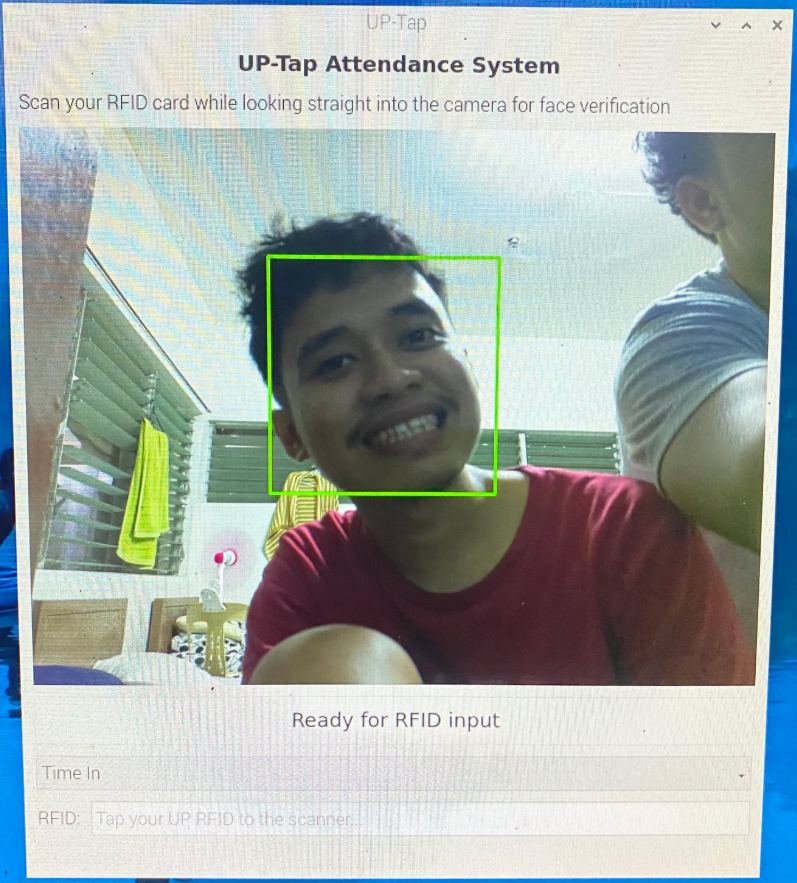
\includegraphics[width=0.75\textwidth]{figures/chapter4/ai_cam_app.png} % Adjust width as needed
	\caption{The camera app running the face detection model}
	\label{fig:ai_cam_app}
\end{figure}
\section{MobileFacenet in detail}
The MobileFacenet model for was used face verification. The model takes in a 112x112x3 image and outputs an embedding(a mathematical representation of face). We then use Cosine similarity with a certain threshold to compute if two embeddings are similar, therefore concluding that both identities are the same. The model was converted to a Tensorflowlite model to run faster on the Raspberry Pi 5 hardware. The final size of the model is 863Kb.

\subsection{Model Architecture}
Figure \ref{fig:mfn_arch} Shows the general architecture of the model as defined in the MobileFacenet paper \cite{chen2018mobilefacenets}.
\begin{figure}[h] % 'h' places the figure approximately here in the text
	\centering
	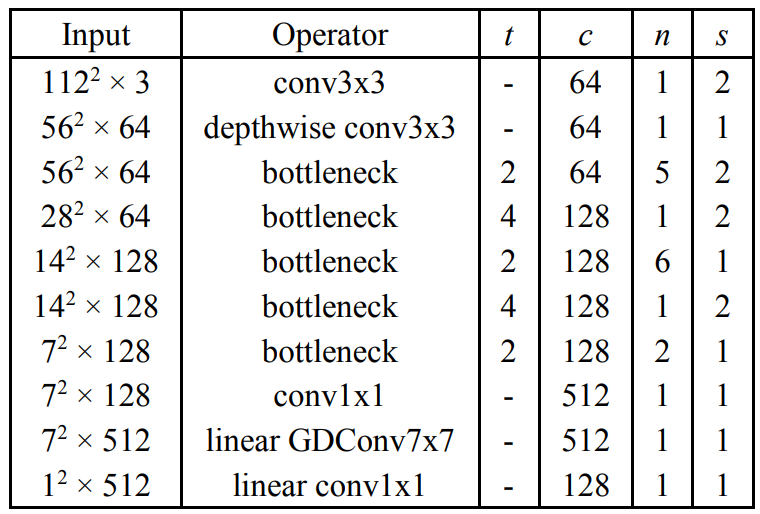
\includegraphics[width=0.5\textwidth]{figures/chapter4/mfn_arch.png} % Adjust width as needed
	\caption{MobileFaceNet Architecture}
	\label{fig:mfn_arch}
\end{figure}

\clearpage 
\subsection{Metrics}
We tested the discriminative ability of the model using the Labeled Faces in the Wild (LFW) Dataset via sklearn. The dataset includes 13,233 images of 5,749 people. The sklearn package provides a 300 pairs of same + 300 pairs of different people per fold. We tested the model in 10 folds.
Compared to models of hundreds of MB in size, the performance of the model is good but can be better. Figure \ref{fig:roc_curve} shows the ROC AUC of the model of 0.77. An Area Under the Curve (AUC) of 0.77 means that if we pick one genuine (same‐person) pair and one impostor (different‐person) pair at random, there’s a 77\% chance the model will score the genuine pair higher.
\begin{figure}[h] % 'h' places the figure approximately here in the text
	\centering
	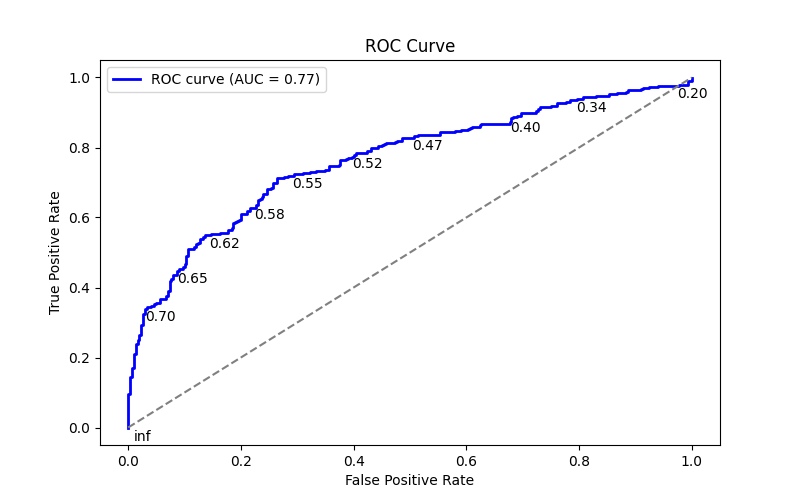
\includegraphics[width=1\textwidth]{figures/chapter4/roc_curve.png} % Adjust width as needed
	\caption{Receiver Operating Characteristic (ROC) Curve for Face Verification}
	\label{fig:roc_curve}
\end{figure}

\clearpage
Next, we evaluate the model's overall accuracy using the chosen threshold. As shown in Figure \ref{fig:fixed_thresh}, the confusion matrix corresponds to a fixed threshold of 0.6. This threshold was selected to strike a practical balance between security (minimizing false positives) and reliability (maintaining acceptable true positive rates). At this setting, the model achieved an average accuracy of 68.6\% across ten cross-validation folds. While this accuracy may not appear high, it is important to note that the evaluated model is a TensorFlow Lite version, optimized and compressed for real-time inference on a Raspberry Pi 5. This compression trades off some performance for significantly improved inference speed on edge devices.
\begin{figure}[h] % 'h' places the figure approximately here in the text
	\centering
	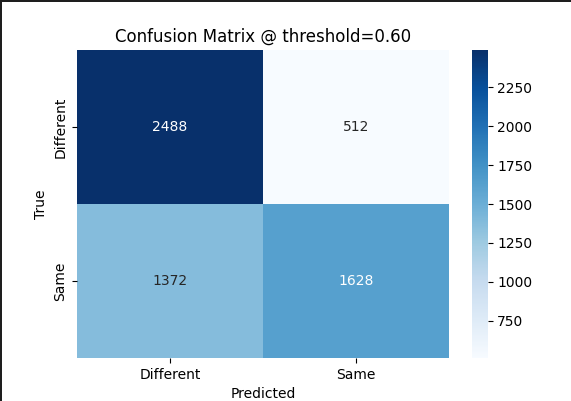
\includegraphics[width=0.75\textwidth]{figures/chapter4/fixed_thresh_matrix.png} % Adjust width as needed
	\caption{Confusion Matrix at a Threshold of 0.60}
	\label{fig:fixed_thresh}
\end{figure}


\section{Mediapipe Face Mesh for a simple face alignment}
To account for the slight misalignment of our camera setup, we implemented a face alignment step next to cropping the facial region. Specifically, we used eye landmarks provided by MediaPipe Face Mesh to estimate the tilt of the face relative to the horizontal axis. The coordinates of the left and right eyes were extracted and used to compute the angle of rotation based on the arctangent of the vertical and horizontal distance between them. The image was then rotated around the midpoint between the eyes using this angle to horizontally align the face. 
This alignment ensures that the cropped facial region remains consistent across samples, improving the robustness of our face verification. After alignment, we calculated the bounding box based on the full set of detected landmarks and cropped the aligned image accordingly. To maintain validity, all bounding box coordinates were clamped to stay within the image boundaries. This preprocessing step proved particularly important for deployment on our Raspberry Pi 5 system, where small variations in camera placement or head orientation could significantly impact performance. Figure \ref{fig:mp_face_mesh} shows the code snippet of our utility function implementing MediaPipe Face Mesh for face alignment. 
\begin{figure}[h] % 'h' places the figure approximately here in the text
	\centering
	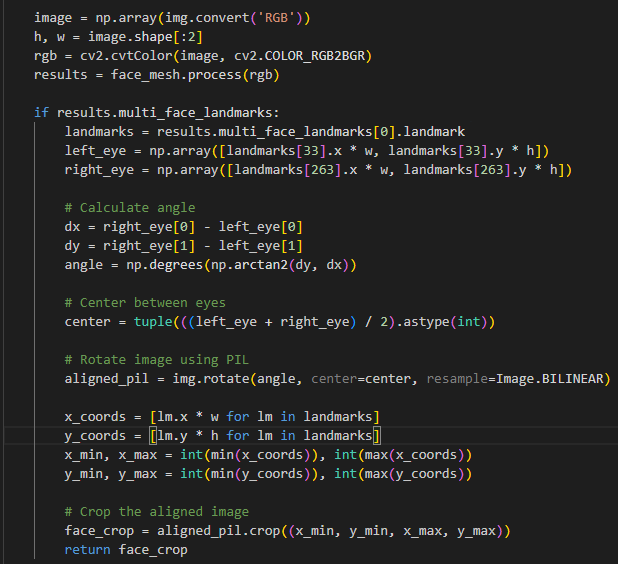
\includegraphics[width=0.75\textwidth]{figures/chapter4/mp_face_mesh.png} % Adjust width as needed
	\caption{}
	\label{fig:mp_face_mesh}
\end{figure}

\clearpage
\section{YoloV8n for Face Detection}
We utilized a pretrained YOLOv8n face detection model developed by Arnab Dhar and published on Hugging Face. This model was fine-tuned by the original author on a dataset of over 10{,}000 face images, trained for 100 epochs using a batch size of 16 on a single NVIDIA V100 16GB GPU (total training time: approximately 140 minutes).

The model achieved the following performance metrics, as reported by the author:

\begin{itemize}
	\item \textbf{Precision (IoU $\geq$ 0.5):} 0.772 ($\approx$77.2\%)
	\item \textbf{Recall (IoU $\geq$ 0.5):} 0.489 ($\approx$48.9\%)
	\item \textbf{mAP@50:} 0.5598 ($\approx$55.98\%)
	\item \textbf{mAP@50--95:} 0.2905 ($\approx$29.05\%)
\end{itemize}


These results demonstrate that the model has strong face detection capabilities, with a good balance between precision and recall. Figure~\ref{fig:yolo-metrics} presents the performance curves for all four metrics across training epochs.

The YOLOv8n model was selected due to its compatibility with the Raspberry Pi AI Camera and the Sony IMX500 edge processor. The Ultralytics framework simplifies quantization and compression via Sony’s Model Compression Toolkit. This enables reducing the model size from around 6~MB to approximately 3~MB, allowing it to run within the IMX500’s 8~MB memory constraint with minimal accuracy loss.

\begin{figure}[H]
	\centering
	\begin{subfigure}[b]{0.48\textwidth}
		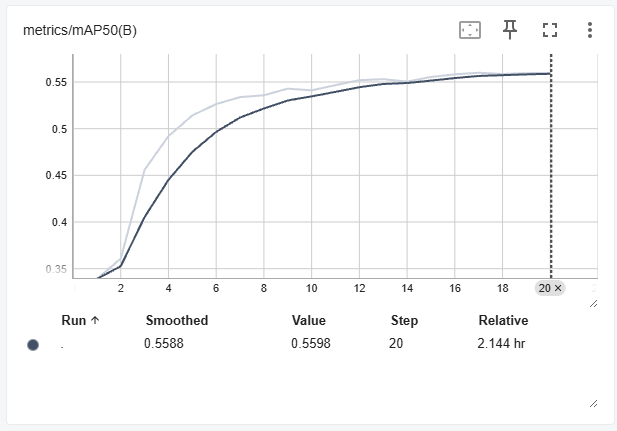
\includegraphics[width=\textwidth]{figures/chapter4/map50.png}
		\caption{mAP@50}
	\end{subfigure}
	\hfill
	\begin{subfigure}[b]{0.48\textwidth}
		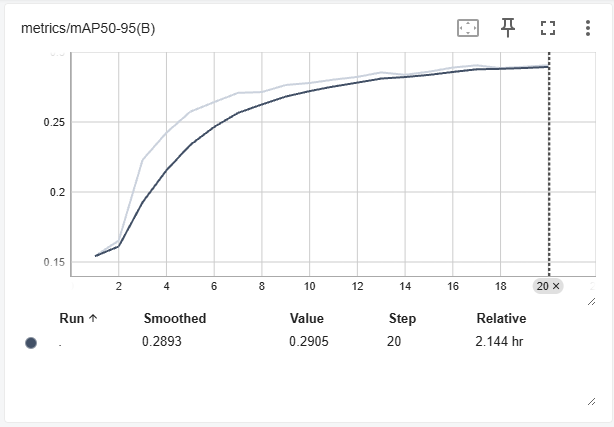
\includegraphics[width=\textwidth]{figures/chapter4/map5095.png}
		\caption{mAP@50--95}
	\end{subfigure}
	
	\vspace{1em}
	
	\begin{subfigure}[b]{0.48\textwidth}
		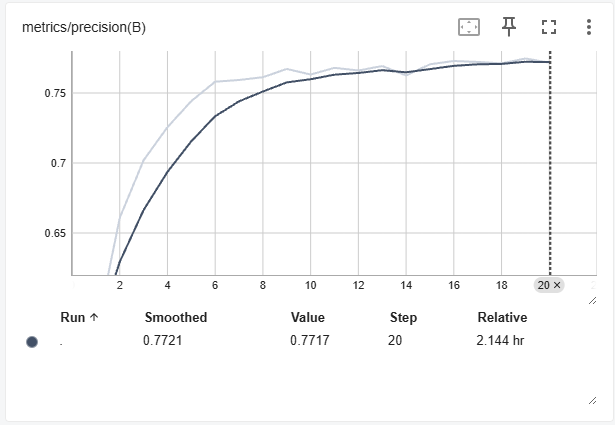
\includegraphics[width=\textwidth]{figures/chapter4/precision.png}
		\caption{Precision (IoU $\geq$ 0.5)}
	\end{subfigure}
	\hfill
	\begin{subfigure}[b]{0.48\textwidth}
		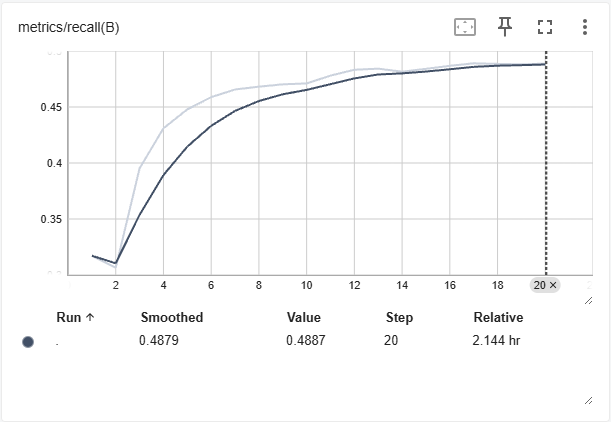
\includegraphics[width=\textwidth]{figures/chapter4/recall.png}
		\caption{Recall (IoU $\geq$ 0.5)}
	\end{subfigure}
	
	\caption{Performance metrics of the YOLOv8n face detection model across training epochs.}
	\label{fig:yolo-metrics}
\end{figure}





